\documentclass{article}
\usepackage[utf8]{inputenc}
\usepackage{geometry}
\usepackage{graphicx}
\usepackage{amsmath}
\usepackage{booktabs}
\usepackage{hyperref}
\usepackage{xcolor}
\usepackage{listings}
\usepackage{caption}
\usepackage{float}
\usepackage{algorithmicx}
\usepackage{algpseudocode}
\usepackage{blindtext}
\usepackage{makecell}

\geometry{a4paper, margin=1in}

\title{Exploring the Audio Modality in Persuasion Modeling\\
for Social Deduction Games}
\author{Alon Bebchuk, 314023516 \and Ohad Rubin, 203184155}
\date{April 15, 2025}

\begin{document}

\maketitle

\begin{abstract}
In this paper, we explore the role of audio modality in persuasion modeling within social deduction games. Building upon previous work that demonstrated the value of multimodal approaches combining text and video, we focus specifically on extracting persuasion strategies from audio data. We compare text-only BERT models with Whisper models that leverage both text and audio features. Our experiments show that Whisper-based models combining audio and text can outperform text-only models by 0.5\% on average F1 score, suggesting that audio features capture beneficial signals for persuasion detection. Our findings indicate that much of the information gained by video modality can be explained by its audio component.
\end{abstract}

\section{Introduction}
Persuasion modeling is a critical component in understanding human communication dynamics and developing conversational agents. Previous research has primarily focused on analyzing persuasion strategies from textual dialogue, with recent advances incorporating visual signals to enhance performance. However, the specific contribution of audio modality in persuasion modeling remains largely unexplored.

Our research builds on the work by Lai et al. \cite{lai2022werewolf}, who introduced a multimodal dataset for modeling persuasion behaviors in social deduction games. They demonstrated that visual cues can improve persuasion strategy prediction by approximately 0.8\% on F1 score compared to text-only models. Our work addresses their call for future research to "explore the role of the audio modality in persuasion modeling and to investigate joint learning of multimodal representations for the social persuasion setting."

We compare text-only models with audio-enhanced approaches, including BERT-based models and Whisper-based models that use both text and audio. Our models are designed to predict persuasion strategies such as Identity Declaration, Accusation, Interrogation, Call for Action, Defense, and Evidence. Through comprehensive experiments, we demonstrate that audio features provide beneficial signals for persuasion detection and can achieve nearly the same performance gains as those previously observed from video data, falling short by only a small margin.

\section{Related Work}
\subsection{Persuasion Modeling}
Research on computational modeling of persuasion has advanced significantly in recent years. Yang et al. \cite{yang2019let} and Chen and Yang \cite{chen2021advisorqagc} introduced datasets focusing on persuasion strategies in online platforms. Chawla et al. \cite{chawla2021casino} examined persuasion in simulated dialogue settings through crowdsourcing. However, these datasets predominantly consist of textual data without incorporating multimodal elements.

\subsection{Multimodal Social Interaction Analysis}
Multimodal approaches to social interaction analysis have gained traction with works like Xu et al. \cite{xu2021learning} and Li et al. \cite{li2020deep} on multimodal sentiment analysis. Bai et al. \cite{bai2021power} applied multimodal methods to predict debate outcomes from TV shows. The Ego4D Social benchmark \cite{grauman2022ego4d} includes tasks for identifying social interactions using video and audio. While these approaches incorporate multiple modalities, they typically do not focus specifically on persuasion strategies.

\subsection{Audio Processing for Social Interaction}
The Whisper model \cite{radford2022robust} represents a significant advancement in audio processing, demonstrating robust speech recognition capabilities across various domains. Recent work has begun exploring Whisper's potential for social interaction understanding beyond simple transcription, though its application to persuasion modeling remains novel.

\subsection{Computational Modeling of Deduction Games}
Previous research has explored computational models for social deduction games, with Chittaranjan and Hung \cite{chittaranjan2010you} developing a model for predicting Werewolf game outcomes based on speaking patterns. However, our work uniquely focuses on understanding persuasive strategies in such games from a multimodal perspective, specifically highlighting the audio component.

\section{Method}
We implement and compare several models to evaluate the contribution of audio modality in persuasion strategy prediction. This section details our model architecture, evaluation metrics, and experimental setup.

\subsection{Architecture}
Our models fall into two main categories: BERT-based text-only models and Whisper-based models that leverage both text and audio.

\subsubsection{BERT-based Models}
\begin{itemize}
    \item \textbf{BERT Single-Task (ST):} We fine-tune separate binary classifiers for each persuasion strategy using the BERT-base-uncased model. Each classifier takes as input a prompt containing the strategy definition, previous utterances (context), and the target utterance.
    
    \item \textbf{BERT Multi-Task Binary-Label (MTBL):} Similar to the single-task model, but we train a single model that can predict any strategy based on the strategy mentioned in the prompt.
    
    \item \textbf{BERT Multi-Task Multi-Label (MTML):} We train a single model to predict all six persuasion strategies simultaneously. The input is only the previous utterances and target utterance, without any strategy-specific prompt.
\end{itemize}

Figure \ref{fig:bert_st_and_mtbl} shows the architecture of the BERT Single-Task and Multi-Task Binary-Label models, while Figure \ref{fig:bert_mtml} shows the Multi-Task Multi-Label variant.

\begin{figure}[H]
    \centering
    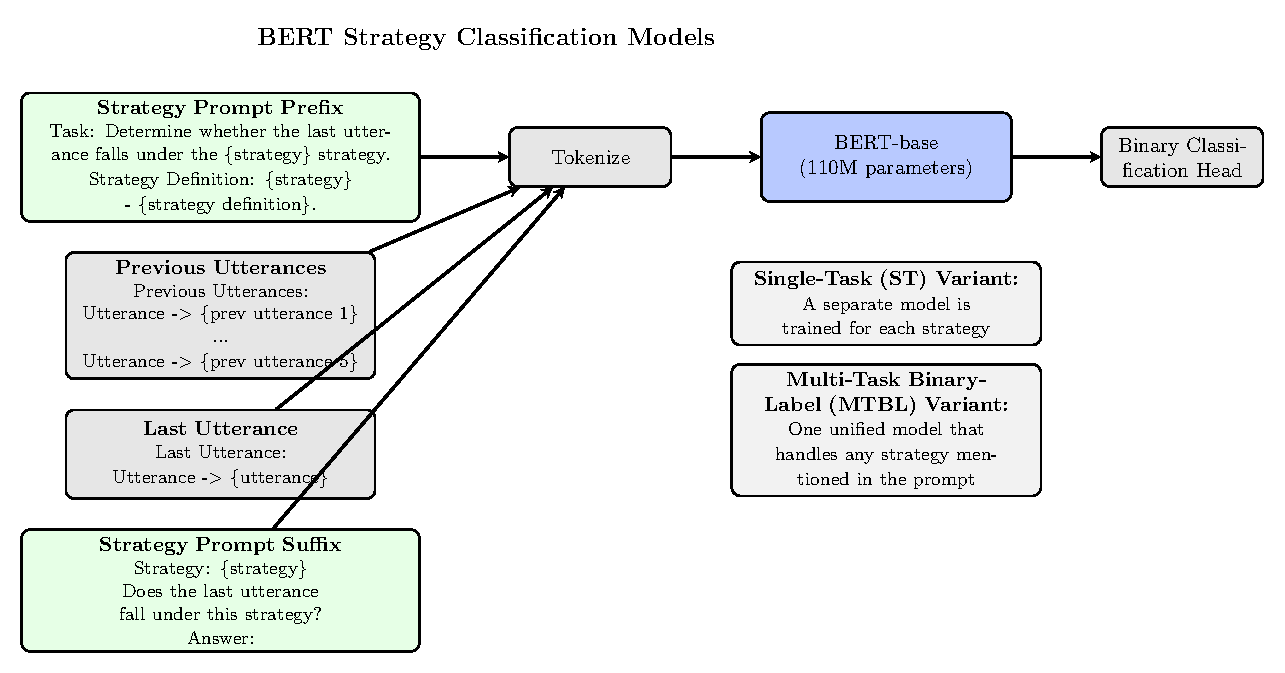
\includegraphics[width=\textwidth]{figures/pdf/bert_st_and_mtbl.pdf}
    \caption{Architecture of the BERT Single-Task (ST) and Multi-Task Binary-Label (MTBL) models. The ST variant uses a separate model for each of the six persuasion strategies, while the MTBL variant uses a single model that handles all strategies based on which one is specified in the prompt.}
    \label{fig:bert_st_and_mtbl}
\end{figure}

\begin{figure}[H]
    \centering
    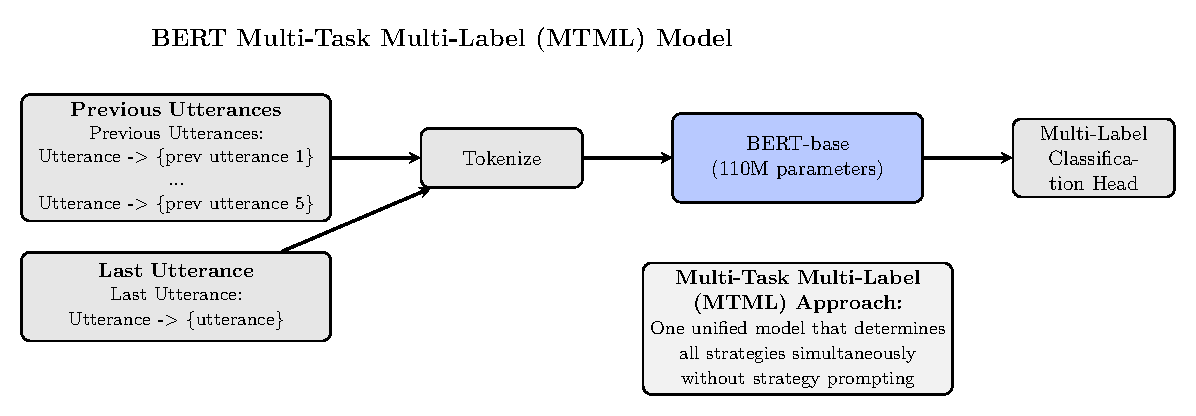
\includegraphics[width=\textwidth]{figures/pdf/bert_mtml.pdf}
    \caption{Architecture of the BERT Multi-Task Multi-Label (MTML) model. A single model simultaneously predicts all six strategies without strategy-specific prompting.}
    \label{fig:bert_mtml}
\end{figure}

\subsubsection{Whisper-based Models}
\begin{itemize}
    \item \textbf{Whisper Yes-No (YN) Models:} We fine-tune the Whisper-small model to generate a "yes" or "no" response to indicate whether the target utterance exhibits the strategy. We implement two variants:
    \begin{itemize}
        \item \textbf{Single-Task (YN ST):} A separate model for each strategy
        \item \textbf{Multi-Task Binary-Label (YN MTBL):} A single model for all strategies, where the strategy is specified in the prompt
    \end{itemize}
    
    \item \textbf{Whisper Projection Models:} We extend the Whisper-small model with a projection layer that transforms the last token's logits, followed by a dropout layer and a classification head. We implement three variants:
    \begin{itemize}
        \item \textbf{Single-Task (Proj ST):} A separate model for each strategy
        \item \textbf{Multi-Task Binary-Label (Proj MTBL):} A single model for all strategies, where the strategy is specified in the prompt
        \item \textbf{Multi-Task Multi-Label (Proj MTML):} A single model that predicts all strategies simultaneously without strategy-specific prompting
    \end{itemize}
\end{itemize}

All Whisper-based models are trained on both text and audio data, where the audio input corresponds to the utterances in the dialogue context. Figures \ref{fig:whisper_yn_st_and_mtbl}, \ref{fig:whisper_proj_st_and_mtbl}, and \ref{fig:whisper_proj_mtml} show the architectures of these models.

\begin{figure}[H]
    \centering
    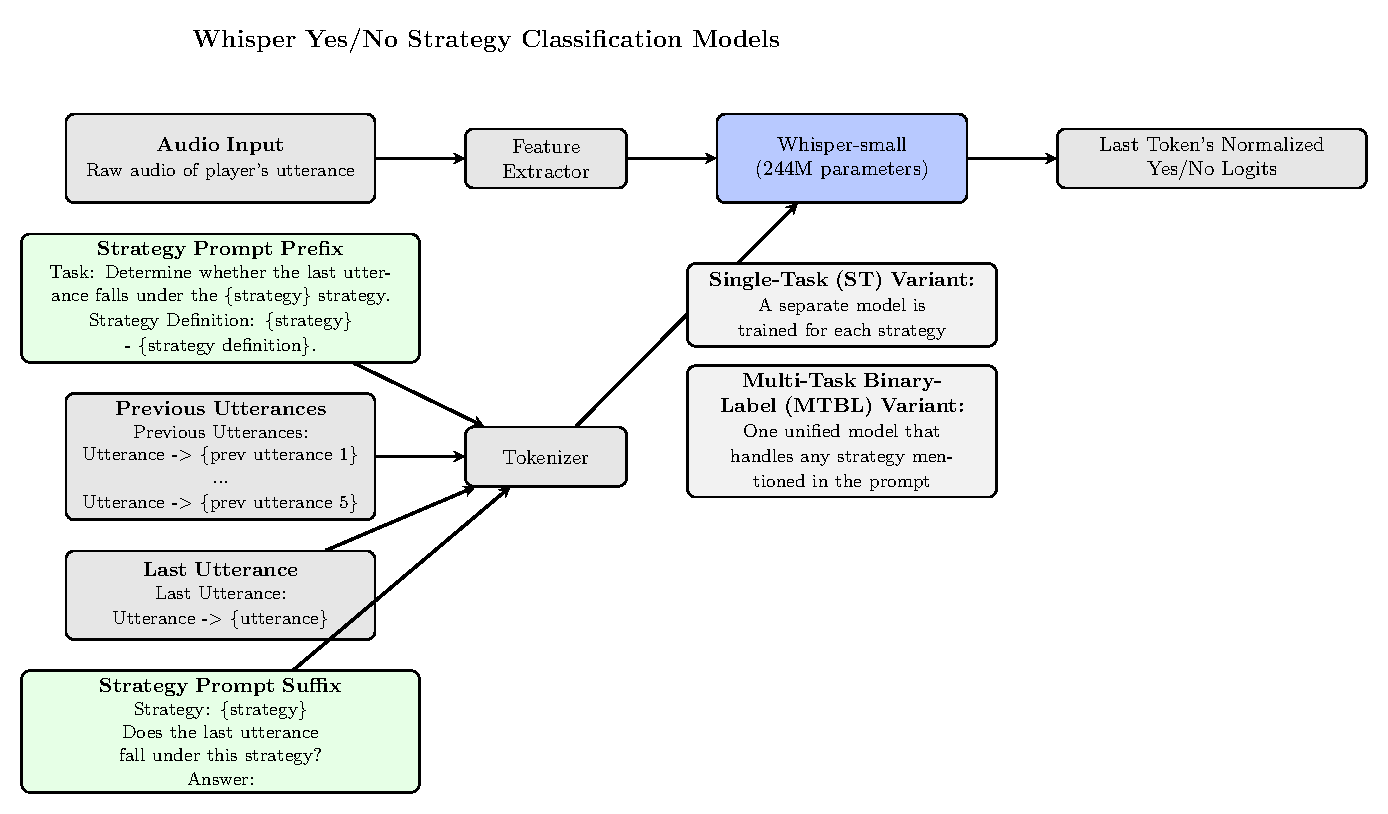
\includegraphics[width=\textwidth]{figures/pdf/whisper_yn_st_and_mtbl.pdf}
    \caption{Architecture of the Whisper Yes-No Single-Task (YN ST) and Multi-Task Binary-Label (YN MTBL) models. These models process both audio and text inputs and use the last token's normalized yes/no logits to predict strategy presence.}
    \label{fig:whisper_yn_st_and_mtbl}
\end{figure}

\begin{figure}[H]
    \centering
    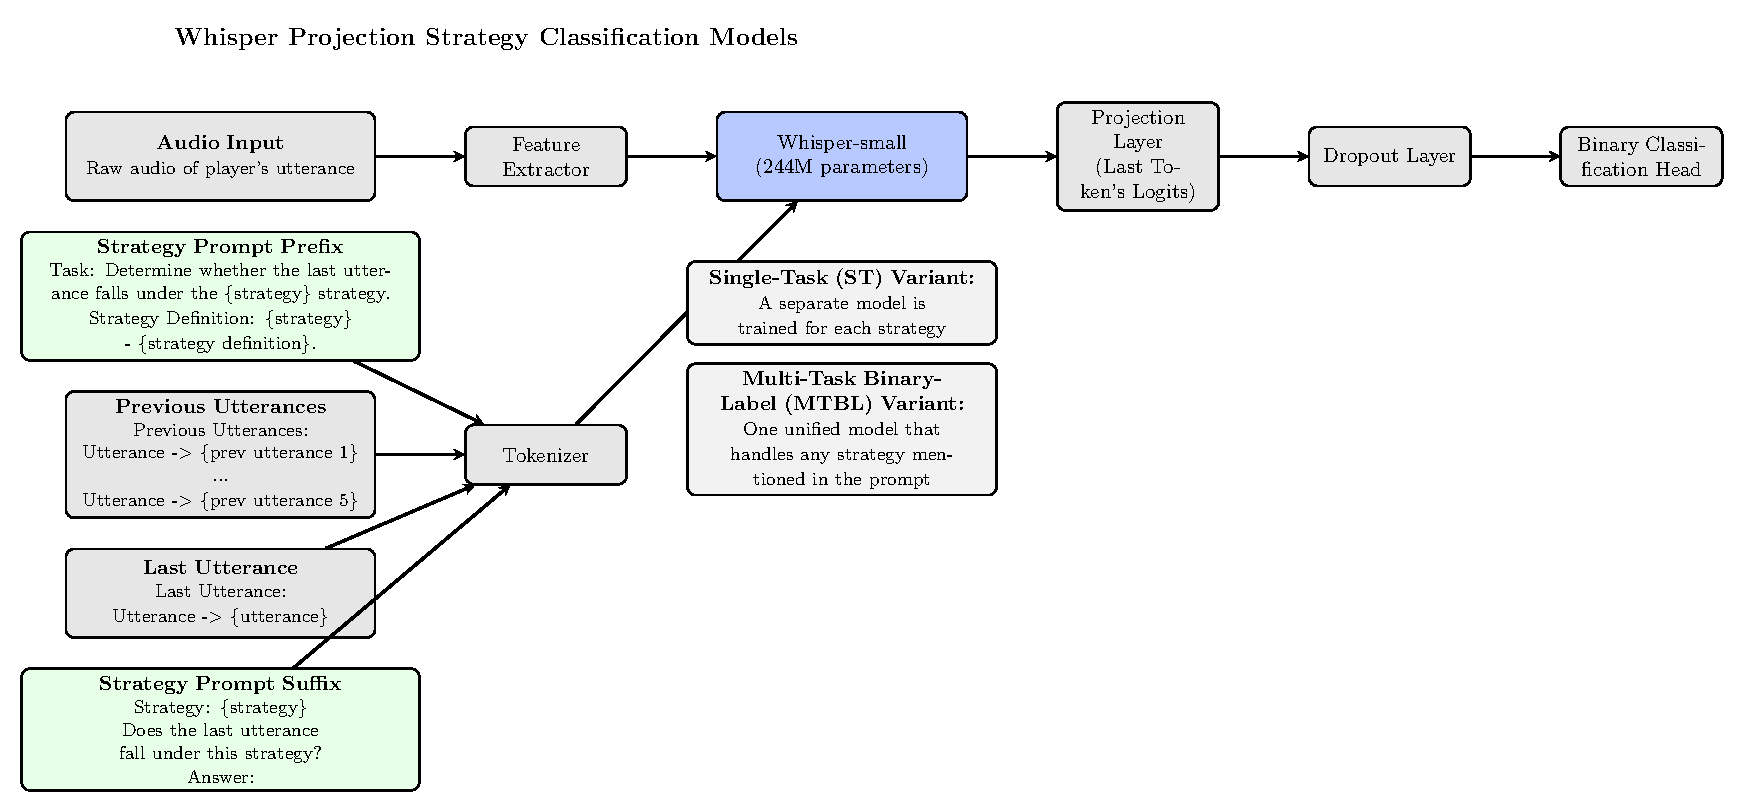
\includegraphics[width=\textwidth]{figures/pdf/whisper_proj_st_and_mtbl.pdf}
    \caption{Architecture of the Whisper Projection Single-Task (Proj ST) and Multi-Task Binary-Label (Proj MTBL) models. These models extend Whisper with additional layers: a projection layer operating on the last token's logits, a dropout layer, and a binary classification head.}
    \label{fig:whisper_proj_st_and_mtbl}
\end{figure}

\begin{figure}[H]
    \centering
    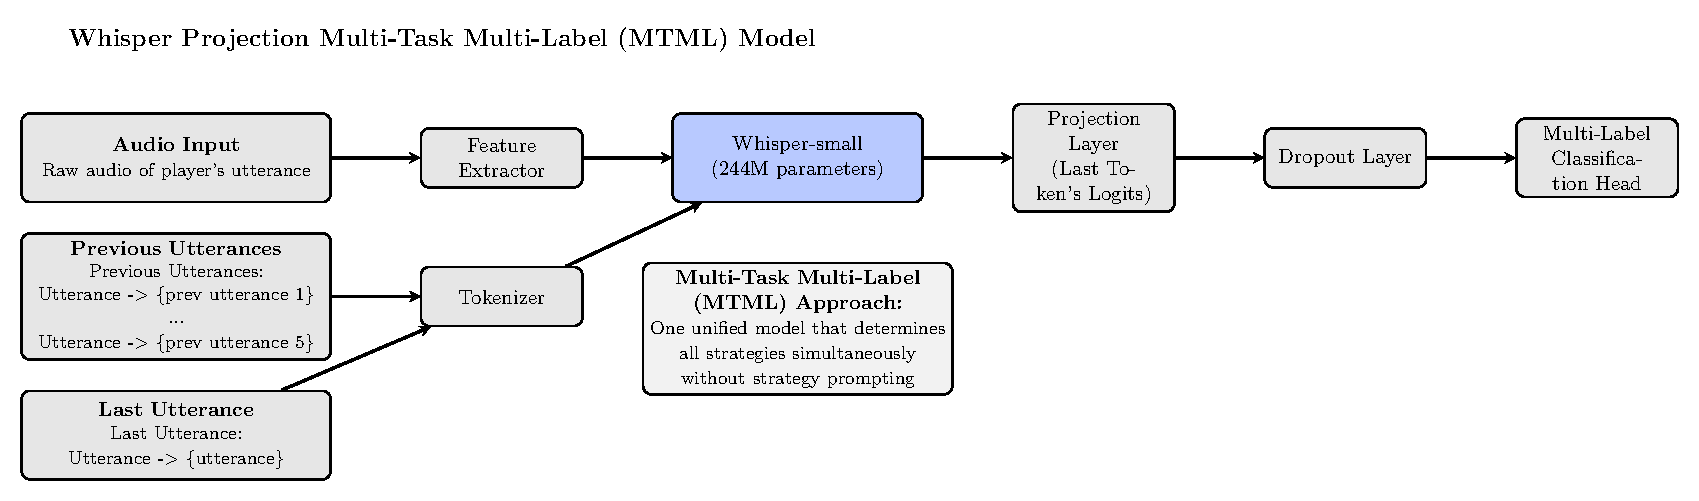
\includegraphics[width=\textwidth]{figures/pdf/whisper_proj_mtml.pdf}
    \caption{Architecture of the Whisper Projection Multi-Task Multi-Label (Proj MTML) model. This model simultaneously predicts all strategies without strategy-specific prompting, using a multi-label classification head.}
    \label{fig:whisper_proj_mtml}
\end{figure}

\subsection{Evaluation Metrics}
Following Chawla et al. \cite{chawla2021casino} and Lai et al. \cite{lai2022werewolf}, we report:
\begin{itemize}
    \item F1 score for each persuasion strategy.
    \item Average F1 score across all strategies.
    \item Accuracy for each persuasion strategy.
    \item Average accuracy across all strategies.
\end{itemize}

\subsection{Experimental Setup}
We use the Werewolf Among Us dataset \cite{lai2022werewolf}, which contains dialogue transcriptions and videos from YouTube of people playing the social deduction game "One Night Ultimate Werewolf." 

\subsubsection{Training Configuration}
\begin{itemize}
    \item Context size: 5 previous utterances (following the optimal setting from Lai et al.)
    \item BERT learning rate: 3e-5
    \item Whisper learning rate: 1e-5, adam $\beta_2$: 0.99, and warmup steps: 200 for stability
    \item Training epochs: 10
    \item Hardware: 8 TPUs
    \item Implementation: JAX/Flax
\end{itemize}

For each model configuration, we train with three different random seeds (12, 42, 87). We evaluate on the validation set every 2 epochs and select the checkpoint with the highest F1 score for final evaluation on the test set.

\section{Results and Discussion}

\subsection{Performance Comparison}
Tables 1 and 2 present the F1 scores and accuracy for all models, respectively, across the six persuasion strategies and on average.

\begin{table}[ht]
\centering
\small
\caption{F1 scores (\%) for each persuasion strategy and average across all strategies}
\setlength{\tabcolsep}{4pt}
\begin{tabular}{@{}lccccccc@{}}
\toprule
Method & ID & ACC & INT & CA & DEF & EVI & Avg \\
\midrule
BERT ST & 80.9±1.0 & 64.7±1.3 & 90.0±0.7 & 75.3±1.3 & 41.9±1.7 & 58.5±1.3 & 68.5±0.5 \\
BERT MTBL & 83.2±0.4 & \textbf{67.7±1.3} & \textbf{90.5±0.1} & 76.5±1.3 & 42.3±3.5 & \textbf{60.1±1.1} & 70.4±0.4 \\
BERT MTML & \textbf{83.5±0.4} & 67.7±0.7 & 90.4±0.2 & 74.9±0.1 & 44.1±0.4 & 57.3±0.5 & 69.7±0.1 \\
Whisper YN ST & 82.8±1.5 & 64.1±1.5 & 89.8±0.6 & \textbf{77.2±0.6} & 47.2±0.5 & 57.7±1.0 & 69.8±0.1 \\
Whisper YN MTBL & 83.4±0.3 & 66.3±0.3 & 90.2±0.2 & 77.1±1.2 & \textbf{48.6±1.6} & 58.5±0.5 & \textbf{70.9±0.3} \\
Whisper Proj ST & 38.4±2.8 & 33.1±1.0 & 51.9±2.0 & 33.8±6.8 & 21.1±2.8 & 25.2±2.5 & 33.9±1.8 \\
Whisper Proj MTBL & 0.0±0.0 & 0.0±0.0 & 0.0±0.0 & 0.0±0.0 & 0.0±0.0 & 0.0±0.0 & 0.0±0.0 \\
Whisper Proj MTML & 34.0±1.2 & 29.2±1.5 & 51.0±1.5 & 28.3±2.1 & 24.2±1.3 & 21.9±2.0 & 31.5±0.4 \\
\bottomrule
\end{tabular}
\parbox{\textwidth}{\small ID: Identity Declaration, ACC: Accusation, INT: Interrogation, CA: Call for Action, DEF: Defense, EVI: Evidence}
\end{table}

\begin{table}[ht]
\centering
\small
\caption{Accuracy (\%) for each persuasion strategy and average across all strategies}
\setlength{\tabcolsep}{4pt}
\begin{tabular}{@{}lccccccc@{}}
\toprule
Method & ID & ACC & INT & CA & DEF & EVI & Avg \\
\midrule
BERT ST & 97.7±0.2 & 89.4±0.4 & 96.1±0.2 & 96.2±0.2 & 83.1±0.6 & 92.8±0.3 & 92.6±0.1 \\
BERT MTBL & 98.1±0.1 & 89.5±0.8 & \textbf{96.3±0.0} & 96.4±0.3 & 84.5±1.4 & 92.6±0.2 & 92.9±0.3 \\
BERT MTML & 98.0±0.0 & \textbf{90.0±0.1} & 96.3±0.1 & 96.2±0.1 & 83.5±0.7 & 92.3±0.1 & 92.7±0.6 \\
Whisper YN ST & 98.1±0.2 & 89.1±0.1 & 96.0±0.2 & \textbf{96.6±0.1} & 84.4±0.6 & \textbf{93.0±0.2} & 92.9±0.1 \\
Whisper YN MTBL & \textbf{98.1±0.0} & 89.9±0.2 & 96.2±0.1 & 96.6±0.1 & 85.5±0.1 & 92.4±0.1 & \textbf{93.1±0.0} \\
Whisper Proj ST & 94.5±0.3 & 82.4±0.7 & 83.6±0.5 & 92.4±0.4 & 83.5±0.3 & 88.4±1.1 & 87.5±0.4 \\
Whisper Proj MTBL & 94.1±0.0 & 84.7±0.0 & 80.7±0.0 & 92.3±0.0 & \textbf{85.7±0.0} & 90.4±0.0 & 88.0±0.0 \\
Whisper Proj MTML & 94.2±0.1 & 81.8±0.7 & 83.6±0.3 & 92.2±0.2 & 83.5±0.2 & 89.4±0.3 & 87.5±0.4 \\
\bottomrule
\end{tabular}
\parbox{\textwidth}{\small ID: Identity Declaration, ACC: Accusation, INT: Interrogation, CA: Call for Action, DEF: Defense, EVI: Evidence}
\end{table}

\subsection{Key Findings}
\begin{itemize}
    \item \textbf{Audio improves persuasion detection:} The Whisper Yes-No Multi-Task Binary-Label model achieves the best average performance with 70.9\% average F1 score and 93.1\% average accuracy, outperforming the best BERT F1 and accuracy models (BERT MTBL and BERT MTML) by 0.5\% average F1 score and 0.2\% average accuracy, respectively.
    
    \item \textbf{Audio vs. Visual modality:} In the original paper by Lai et al., incorporating visual features improved average F1 score by 0.8\%. Our results suggest that much of this improvement can be attributed to the audio component.
    
    \item \textbf{Multi-task learning effectiveness:} Both for BERT and Whisper models, multi-task approaches generally outperform single-task models, indicating that joint learning across strategies is beneficial.
    
    \item \textbf{Strategy-specific insights:} Audio features seem particularly helpful for "Defense" strategy detection, with a 6.3\% gain in F1 score compared to the best BERT model (48.6\% vs. 44.1\%).
    
    \item \textbf{Projection approach limitations:} The Whisper Projection models performed poorly compared to the Yes-No models. This is likely because Whisper is fundamentally a generative model, and adapting it for classification with a projection layer requires significantly more training data and careful hyperparameter tuning than our experimental setup provided. The Yes-No approach better leverages Whisper's generative capabilities without requiring extensive architectural modifications.
\end{itemize}

\subsection{Analysis}
The improved performance of the Whisper Yes-No models indicates that audio features capture important cues for persuasion detection. These cues might include tone, emphasis, pauses, and other paralinguistic features that are absent in text-only representations. The particularly strong improvement for the "Defense" strategy suggests that audio features may be especially relevant when people are defending themselves or others, as emotional cues in voice can signal credibility and conviction.

The poor performance of the Whisper Projection models highlights the challenges in adapting generative pre-trained models for classification tasks. Whisper was primarily trained for speech recognition in a generative manner, and repurposing it for classification through projection layers requires retraining parts of the model architecture. In contrast, the Yes-No approach fits more naturally with Whisper's generative training objective, as it simply requires the model to generate a specific token ("yes" or "no"). Future work could explore more extensive pretraining and optimization strategies for the projection-based approaches.

\section{Future Work}
Future research could explore several promising directions:

\subsection{Improved Audio Representation Learning}
The Whisper Projection models performed poorly, suggesting room for improvement in how audio representations are used for classification tasks. Future work could investigate:
\begin{itemize}
    \item Pre-training specialized audio encoders on persuasion-specific tasks
    \item Exploring alternative fusion mechanisms between audio and text features
    \item Using contrastive learning to align audio and text representations in a shared embedding space
\end{itemize}

\subsection{Fine-grained Audio Feature Analysis}
A detailed analysis of which audio features contribute most to persuasion strategy detection could provide insights into the mechanism behind the performance of such models. This might involve:
\begin{itemize}
    \item Ablation studies on different audio features (pitch, energy, speech rate)
    \item Attention visualization to identify when the model attends to audio versus text
    \item Probing experiments to understand what persuasion-relevant information is encoded in different layers
\end{itemize}

\subsection{Cross-domain Application}
Testing the audio-enhanced persuasion models on other domains could help understand their generalizability:
\begin{itemize}
    \item Political debates
    \item Sales negotiations
    \item Therapeutic conversations
\end{itemize}

\section{Limitations \& Broader Impact}
\subsection{Limitations}
\begin{itemize}
    \item \textbf{Dataset specificity:} Our models are trained and evaluated on the Werewolf Among Us dataset, which features a specific game setting that may not generalize to other conversational contexts.
    
    \item \textbf{Hyperparameter tuning:} The Whisper Projection models might perform better with extensive hyperparameter tuning, which was beyond the scope of this study.
    
    \item \textbf{Computational requirements:} Training Whisper-based models requires significant computational resources, making thorough hyperparameter optimization and architecture search prohibitively expensive. This limits our ability to fully explore potential modifications that might improve performance.
\end{itemize}

\subsection{Broader Impact}
\begin{itemize}
    \item \textbf{Positive applications:} Models that detect persuasion strategies from multimodal inputs could enhance communication training, assist negotiation coaching, and improve conversational agents' authenticity.
    
    \item \textbf{Potential risks:} The same technology could be misused for manipulation detection avoidance, targeted persuasion, and more. Careful ethical guidelines should accompany deployment of such models.
    
    \item \textbf{Privacy considerations:} Audio analysis raises privacy concerns beyond text analysis, as voice contains biometric information and potentially sensitive paralinguistic cues.
    
    \item \textbf{Bias and fairness:} Persuasion strategies vary across cultures and demographics, and models may perform differently across speaker groups, potentially reinforcing biases if deployed without consideration for diverse populations.
\end{itemize}

\subsection{Ethical Considerations}
As noted by Lai et al., persuasion skills can be used for both beneficial and harmful purposes. Our research aims to understand human behavior in social settings rather than to encourage deception or manipulation. Applications of this technology should be subject to ethical review and appropriate safeguards.

\bibliographystyle{plain}

\begin{thebibliography}{10}

\bibitem{lai2022werewolf}
Lai, B., Liu, Z., Tong, M., Zhou, Y., Yu, Z., Wang, W.Y. (2022). Werewolf Among Us: A Multimodal Dataset for Modeling Persuasion Behaviors in Social Deduction Games. arXiv preprint arXiv:2212.08279.

\bibitem{chawla2021casino}
Chawla, P., Young, D., Jiang, A.X., Zhu, J. (2021). CASINO: Modeling Persuasion Strategies in Peer-to-Peer Interactions. In Proceedings of the 2021 Conference on Empirical Methods in Natural Language Processing.

\bibitem{yang2019let}
Yang, D., Chen, J., Yang, Z., Jurafsky, D., Hovy, E. (2019). Let's Make Your Request More Persuasive: Modeling Persuasive Strategies via Semi-Supervised Neural Nets on Crowdfunding Platforms. In Proceedings of the 2019 Conference of the North American Chapter of the Association for Computational Linguistics.

\bibitem{chen2021advisorqagc}
Chen, J., Yang, D. (2021). AdvisorQA: A Knowledge-Guided Conversational System for Fund Recommendation. In Findings of the Association for Computational Linguistics: EMNLP 2021.

\bibitem{xu2021learning}
Xu, P., Ye, Z., Zhang, J., Li, Y., Tang, S., Wu, F., Lin, Y., Xu, M., Li, Z. (2021). Learning to discrete multifunctional expression for multimodal sentiment analysis. In Proceedings of the 59th Annual Meeting of the Association for Computational Linguistics.

\bibitem{li2020deep}
Li, W., Zhang, W., Zhang, Y., Qian, S., Liao, X., Cao, G., Chen, J. (2020). Deep multimodal fusion for sentiment analysis in videos. In Proceedings of the 2020 Conference on Empirical Methods in Natural Language Processing.

\bibitem{bai2021power}
Bai, H., Chen, M., Liu, Y. (2021). The Power of Nonlinguistic Cues: Analyzing Multimodal Political Debates Using Contextualized Cross-Modal Representations. In International Conference on Learning Representations.

\bibitem{grauman2022ego4d}
Grauman, K., Westbury, A., Byrne, E., Chavis, Z., Furnari, A., Girdhar, R., ... \& Buch, S. (2022). Ego4D: Around the world in 3,000 hours of egocentric video. In Proceedings of the IEEE/CVF Conference on Computer Vision and Pattern Recognition.

\bibitem{radford2022robust}
Radford, A., Kim, J.W., Xu, T., Brockman, G., McLeavey, C., Sutskever, I. (2022). Robust Speech Recognition via Large-Scale Weak Supervision. arXiv preprint arXiv:2212.04356.

\bibitem{chittaranjan2010you}
Chittaranjan, G., Hung, H. (2010). Are you a werewolf? detecting deceptive roles and outcomes in a conversational role-playing game. In IEEE International Conference on Acoustics, Speech and Signal Processing.

\end{thebibliography}

\end{document} 